% ============================================================
% Ejercicio 3
% ============================================================
\section{Ejercicio 3}

\begin{tcolorbox}[enunciado]
Considera el siguiente acertijo.

Bruno, Juan y Samuel trabajan en una ciudad como bombero, policía y maestro, aunque no necesariamente en ese orden.

En la ciudad se rumora lo siguiente:
\begin{itemize}[leftmargin=*]
    \item Bruno y el maestro son vecinos
    \item Juan y el maestro son vecinos
    \item Bruno y Samuel (ambos) son vecinos del bombero
    \item El policía y el bombero (ambos) son vecinos de Juan
    \item Todos son vecinos entre sí
\end{itemize}

Se sabe que solo dos de estas afirmaciones son verdaderas. ¿Qué oficio desempeña cada uno?
\end{tcolorbox}

\begin{enumerate}[label=\arabic*., leftmargin=*]
    \item Expresa el acertijo anterior como un ejemplar concreto de algún problema en NP; Enuncia el problema en su versión canónica. \\
    \textbf{Nota:} Si el problema elegido no es uno de los vistos en clase, demuestra que el problema está en NP.
    
    \subsection*{Solución}
    Primero sabemos por las proposiciones que la ultima sucede, pues todos son vecinos, sin embargo, sucede que el policia y el bombero son vecinos de Juan, de este modo 
    
    \textit{Nota: Si el problema elegido no es uno de los vistos en clase, demuestra que el problema está en $\text{NP}$.}\\

    Se pueden tener varias proposiciones logicas para este problema; visto de esta forma, se tiene la siguiente estructura:
    \begin{enumerate}
        \item $p \rightarrow   q$
        \item $m \rightarrow   q$
        \item $B \wedge S \rightarrow  b$
        \item $p \wedge b \rightarrow  J$
        \item $b \wedge q \wedge p$
    \end{enumerate}

    El problema puede ser visto como un problema de proposiciones logicas, ya que se busca que dos de las afirmaciones sean ciertas o satisfacibles del conjunto de proposiciones.\\

    De la misma manera, dado que son 3 personas, se le puede asignar un posible oficio a cada una de ellas para determinar cual es el verdadero.

    $$Bm,Bp,Bb,Sm,Sp,Sb,Jm,Jp,Jb$$
    
    Por lo que el ejemplar para las proposiciones anteriores seria el siguiente:\\

    \textbf{Ejemplar concreto de SAT (Opcion 1)}\\
    \textbf{Datos:} Proposiciones logicas en conjuncion booleana, $p \rightarrow   q$, $m \rightarrow   q$, $B \wedge S \rightarrow  b$, $p \wedge b \rightarrow  J$, $b \wedge q \wedge p$\\
    \textbf{Respuesta:} $(\neg p \vee q) \wedge (\neg m \vee q) \wedge (\neg B \vee \neg S \vee b) \wedge (\neg p \vee \neg b \vee J) \wedge (b \wedge q \wedge p) = 1$ \\

    Para la solución única del acertijo, definimos los valores de verdad de las variables atómicas según las profesiones asignadas:

\begin{itemize}
    \item $p = 0$: Bruno no es policía; el policía es Juan.
    \item $m = 0$: Juan no es maestro; el maestro es Bruno.
    \item $b = 0$: Juan no es bombero; el bombero es Samuel.
    \item $q = 1$: Todos son vecinos entre sí.
    \item $B = 1$, $S = 1$, $J = 1$: Representan la presencia de Bruno,
    Samuel y Juan como entidades distintas.
\end{itemize}
    Por lo que al evaluarlas tenemos lo siguiente:
    \begin{enumerate}
\item $p \rightarrow q \equiv 0 \rightarrow 1 \equiv 1 \quad \text{(Verdadero)}$
\item $m \rightarrow q \equiv 0 \rightarrow 1 \equiv 1 \quad \text{(Verdadero)}$
\item $B \wedge S \rightarrow b \equiv (1 \wedge 1) \rightarrow 0 \equiv 1 \rightarrow 0 \equiv 0 \quad \text{(Falso)}$
\item $p \wedge b \rightarrow J \equiv (0 \wedge 0) \rightarrow 1 \equiv 0 \rightarrow 1 \equiv 1 \quad \text{(Verdadero)}$
\item $b \wedge q \wedge p \equiv 0 \wedge 1 \wedge 0 \equiv 0 \quad \text{(Falso)}$
\end{enumerate}

    De esta forma Bruno = Maestro, Juan = Policía, Samuel = Bombero, y la proposicion e) y b) son las unicas verdaderas.\\

    \textbf{Ejemplar concreto de SAT (Opcion 2)}\\
    \textbf{Datos:} Proposiciones logicas en conjuncion booleana, $\neg Bp$, $\neg Jm$, $\neg Jb$, $\neg Bp \wedge \neg Jm \wedge \neg Jb$, $b \wedge q \wedge p$\\
    \textbf{Respuesta:} $(\neg p \vee q) \wedge (\neg m \vee q) \wedge (\neg B \vee \neg S \vee b) \wedge (\neg p \vee \neg b \vee J) \wedge (b \wedge q \wedge p) = 1$ \\
    Lo definimos como posibles opciones.\\
    \begin{enumerate}
    \item $A_1 \equiv \neg B_m \quad \text{Bruno y el maestro son vecinos } \implies \text{Bruno no es el maestro}$
    \item $A_2 \equiv \neg J_m \quad \text{(Juan y el maestro son vecinos } \implies \text{Juan no es el maestro)}$
    \item $A_3 \equiv (\neg B_b \wedge \neg S_b) \leftrightarrow J_b \quad \text{Bruno y Samuel son vecinos del bombero } \implies \text{El bombero es Juan }$
    \item $A_4 \equiv \neg J_p \wedge \neg J_b \quad \text{(El policía y el bombero son vecinos de Juan } \implies \text{Juan no es policía ni bombero)}$
    \item $A_5 \equiv \text{True} \quad \text{(Todos son vecinos entre sí } \implies \text{Topología completa del vecindario)}$
    \end{enumerate}
    
    Se construye la fórmula proposicional que exige que exactamente dos de las variables $\{A_1, A_2, A_3, A_4, A_5\}$ sean verdaderas y las otras tres sean falsas:$$\Gamma_2 = \bigvee_{1 \le i < j \le 5} \left( A_i \wedge A_j \wedge \bigwedge_{k \notin \{i,j\}} \neg A_k \right)$$

    Por lo tanto para este caso el ejemplar corresponderia a $$\Gamma = \Gamma_1 \wedge \Gamma_2$$, donde $\Gamma_1$ es toda la proposicion que es equivale a encontrar una interpretación $v : \{B_b, \dots, S_m\} \rightarrow \{0, 1\}$ tal que $\Gamma$ sea satisfacible ($\Gamma = 1$). Esto nos dara el mismo resultado que la proposicion anterior, por lo tanto funciona de igual manera.\\
    
    
    \textbf{Forma canonica:}
    \textbf{SAT}\\
    \textbf{Datos:} Un conjunto de variables proposicionales $V = \{x_1, x_2, \dots, x_n\}$ y una fórmula lógica $\Gamma$ expresada como una conjunción booleana de $m$ cláusulas

    $$\Gamma = C_1 \wedge C_2 \wedge \dots \wedge C_m$$, donde cada cláusula $C_i = (l_{i,1} \vee l_{i,2} \vee \dots \vee l_{i,k_i})$ es una disyunción de literales con $l \in \{x_j, \neg x_j\}$.
    \textbf{Pregunta:} ¿Existe algún conjunto de valores $V \rightarrow \{0,1\}$ para los cuales la formula logica en conjunción booleana de $m$ clausulas sea satisfacible, es decir $\Gamma = 1$?\\
    
    (Que yo recuerde si, pero no esta de mas)
    Decimos que $L \in NP \iff \exists M$ Determinista $| \exists x $, $|u| = n^k$  $M(x,a) = 1$. Por lo tanto proponemos un certificado para M\\

    Decimos que $L \in NP \iff \exists M$ Determinista $| \exists x $, $|u| = n^k$  $M(x,a) = 1$.\\

    Proponemos como certificado $u$ una asignación de valores de verdad para las $n$ variables de la fórmula proposicional $x$ de longitud $N$, para saber si es satisfacible, el número de variables $n$ está acotado por la longitud del problema ($n \le N$), su tamaño es consecuentemente polinomial ($\vert{}u\vert{} = O(N)$).

    Proponemos un algoritmo determinista de verificacion $(x,u)$ 
    \begin{verbatim}
        result = 1
        // Evaluar cada cláusula C_i bajo la asignación dada por u
        for (i = 0; i < m; i++):
            eval_clausula = 0
            for cada literal L en la clausula C[i]:
                val = u[L.variable]
                if (L es negado):
                    val = !val
                eval_clausula = eval_clausula || val
            
            result = result && eval_clausula
        
        if (result == 1):
            aceptar
        else:
            rechazar
    \end{verbatim}
    
    Asignarle un valor a cada variable atomica y comprobarlo toma $O(N^2)$ ya que recorrer dos veces las proposiciones y asignarles un valor toma $O(N^2)$, comparaciones dentro del for mas anidado toma $O(N^2)$, en el nivel más interno, se realiza una comparación de igualdad y operaciones booleanas ($\text{AND}, \text{OR}, \text{NOT}$), cada una de las cuales toma tiempo $O(1)$.
    Regresar valores $O(1)$, por lo tanto el algoritmo se ejecuta en un tiempo polinomial. Dado que en ambos escenarios la complejidad está acotada por un polinomio $O(N^k)$ (con $k \le 2$), el algoritmo verificador $M(x, u)$ ejecuta en tiempo polinomial determinista, lo que demuestra que el problema pertenece a la clase $\text{NP}$.\\
    
    De esta manera \textbf{SAT} $\in NP$ para el certificado u.
    
    \item Da una representación visual (diagrama, figura, imagen, etc..) del ejemplar concreto, de acuerdo al problema del inciso anterior.
    
    \subsection*{Solución}
    Se puede mediante graficas representar el problema y cada proposicion.
    \begin{figure}[H]
        \centering
        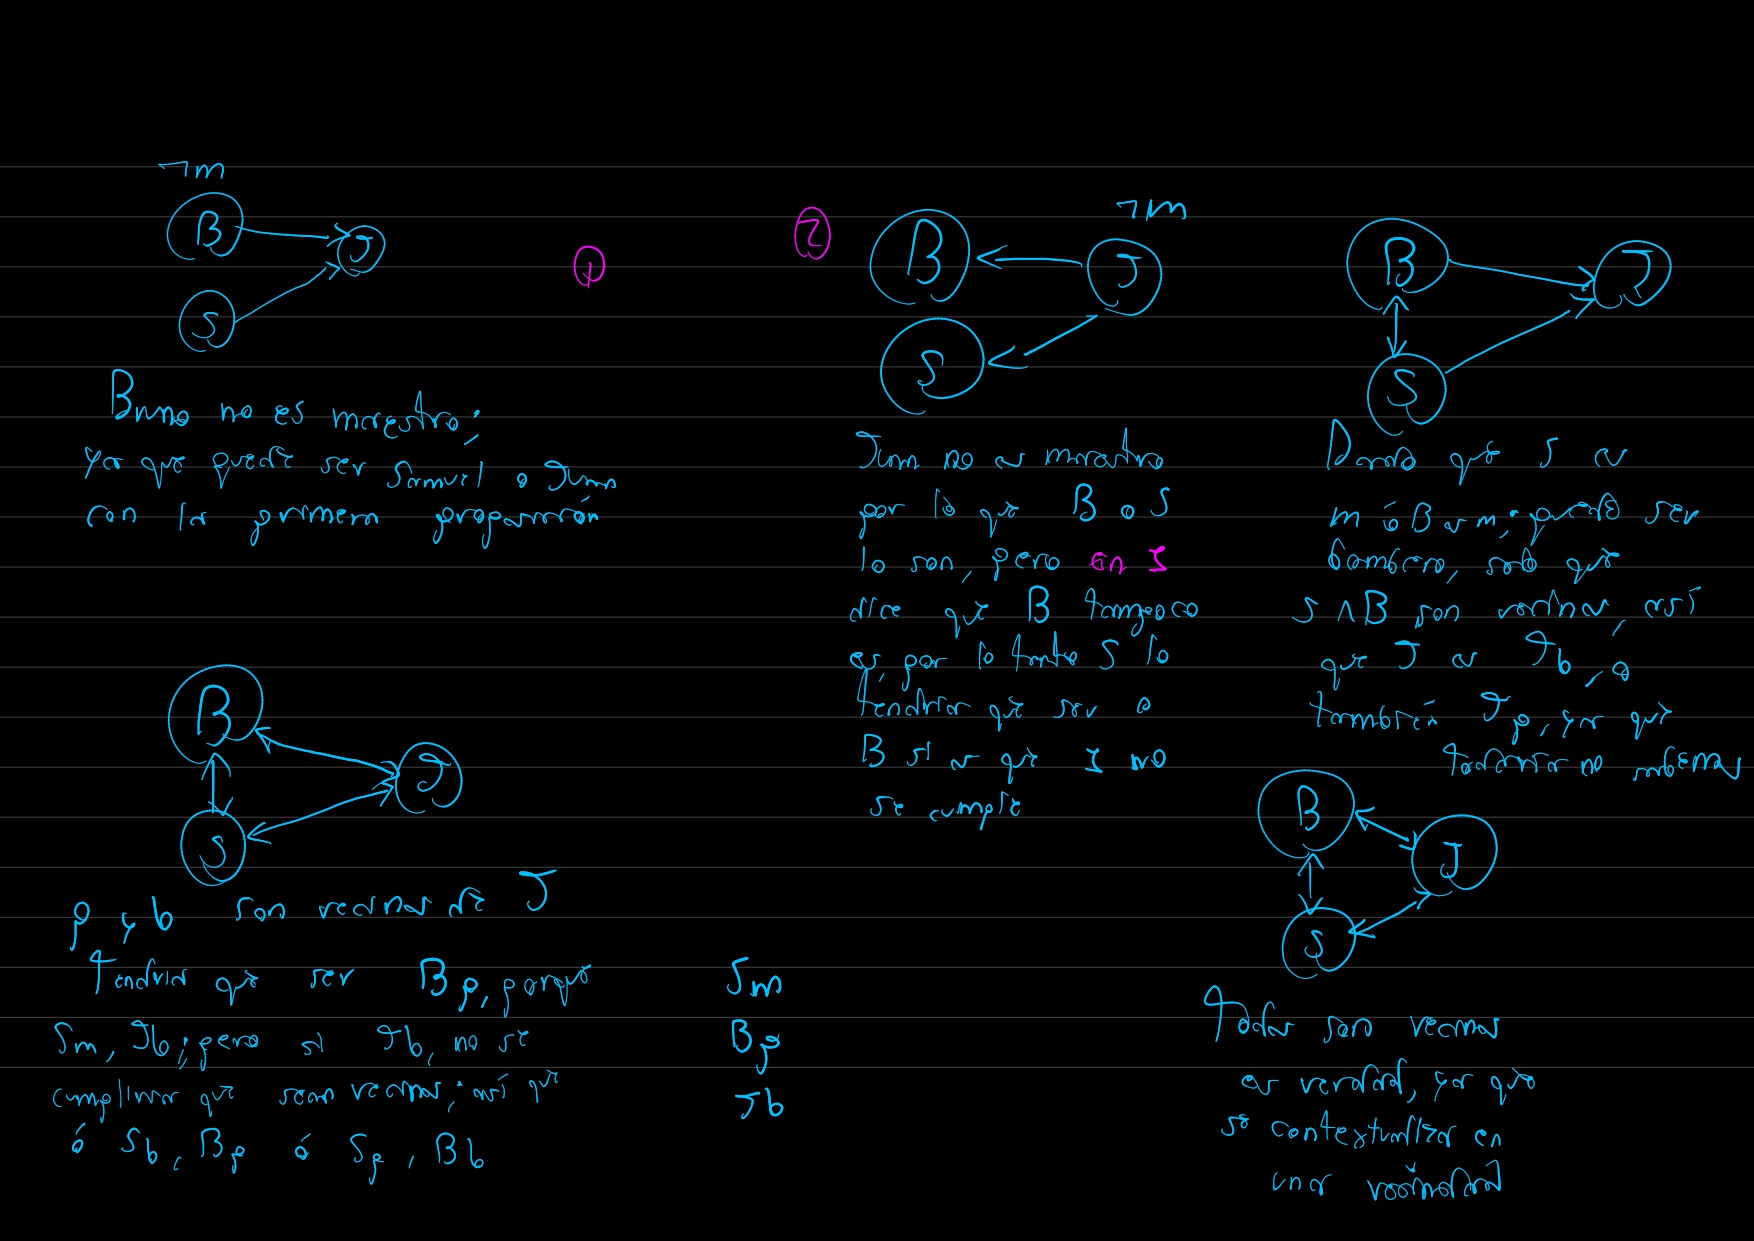
\includegraphics[width=0.8\linewidth]{imagenes/tt.jpg}
    \end{figure}

    \begin{figure}[H]
        \centering
        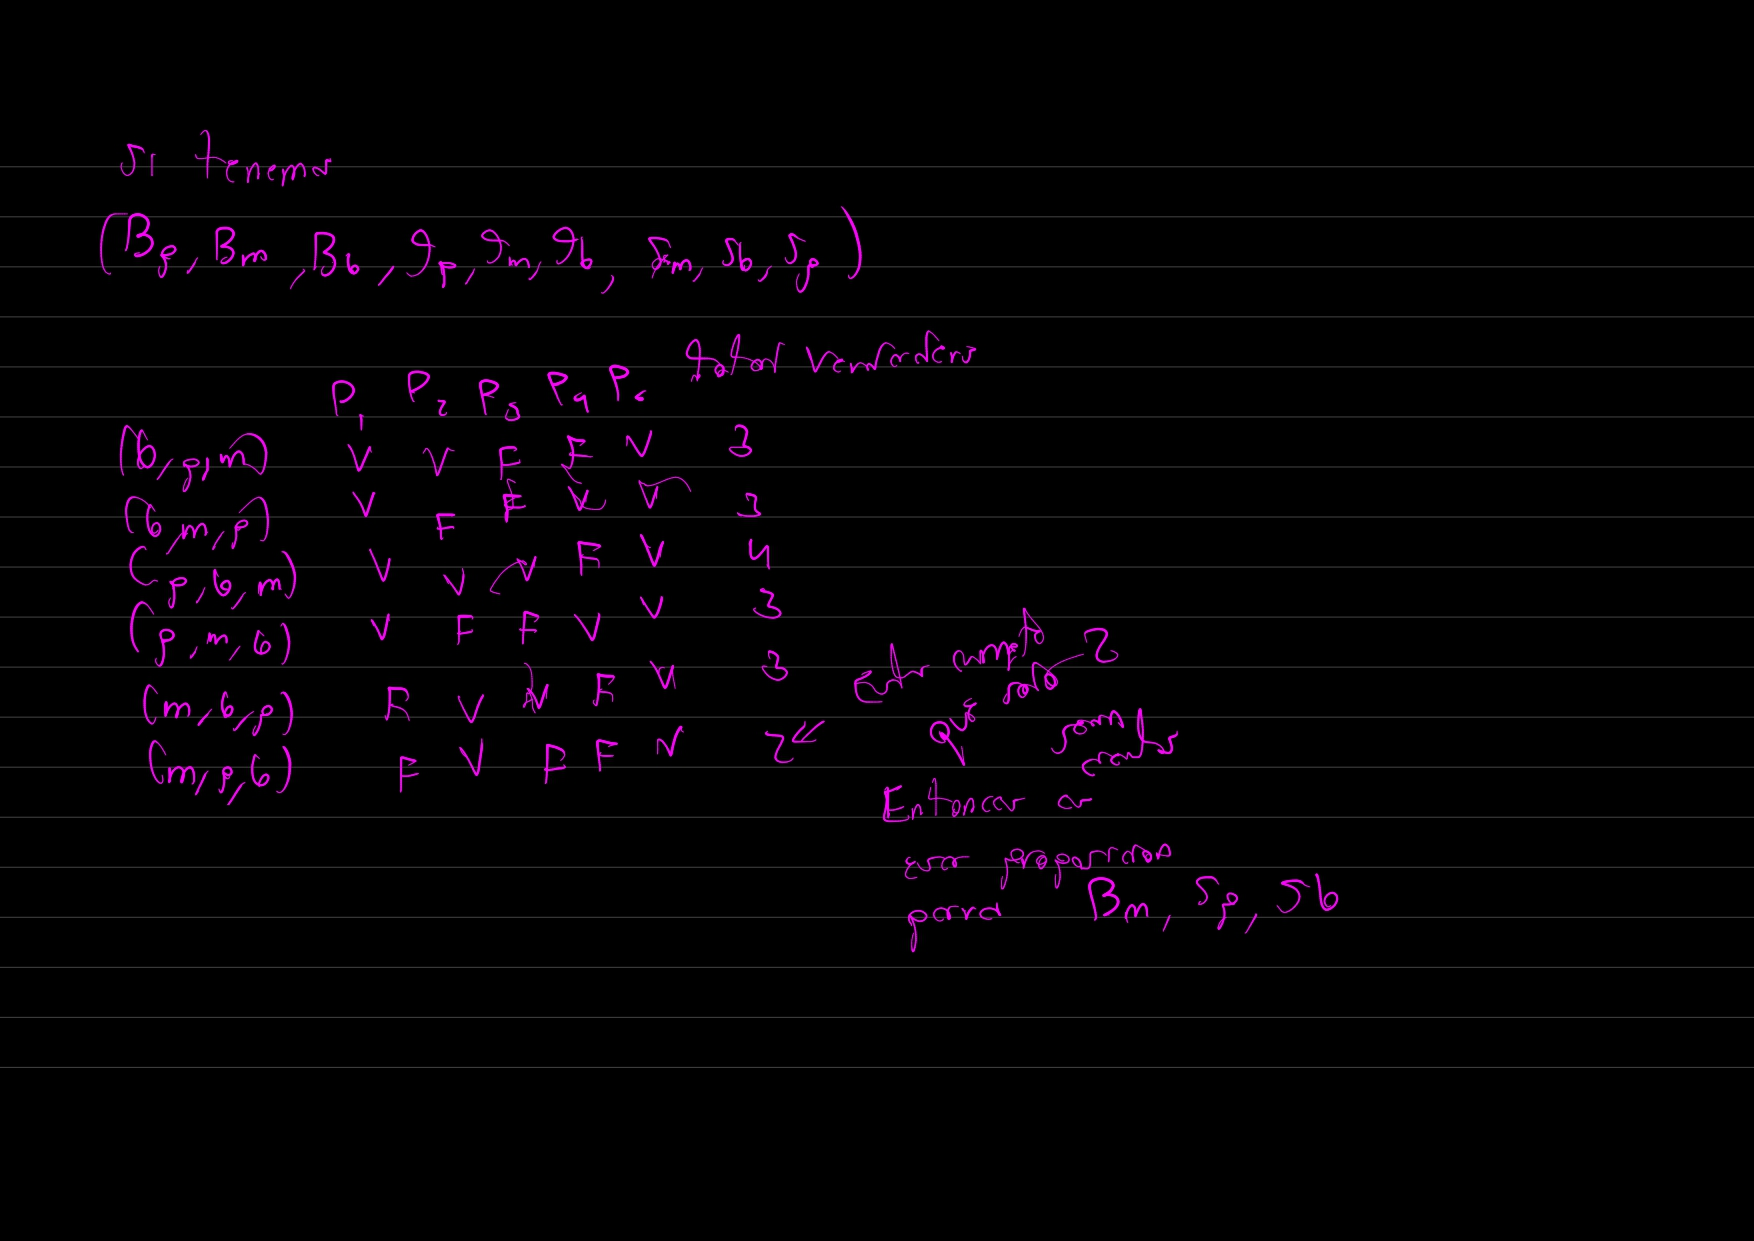
\includegraphics[width=0.8\linewidth]{imagenes/ttt.jpg}
    \end{figure}

    \item Resuelve el acertijo exhibiendo un certificado.
    
    \subsection*{Solución}
    Decimos que $L \in NP \iff \exists M$ Determinista $| \exists x $, $|u| = n^k$  $M(x,a) = 1$.\\

    Definimos el certificado $u$ como el vector binario de asignación de verdad para las 9 variables proposicionales $u = (Bm, Bp, Bb, Jm, Jp, Jb, Sm, Sp, Sb) \in \{0,1\}^9$:$$u = (1, 0, 0, 0, 1, 0, 0, 0, 1)$$

    Esta asignación codifica de forma única los siguientes oficios, Bruno: Maestro ($Bm = 1$)Juan: Policía ($Jp = 1$)Samuel: Bombero ($Sb = 1$)

    Propuesto ya el verificador procesa el certificado $u$ comprobando dos condiciones.\\
    
    Satisfacción de los tipos de oficio de las personas ($\Gamma_1 = 1$)Cada persona tiene un único oficio:$$B_m \vee Bp \vee Bb = 1 \vee 0 \vee 0 = 1$$$$Jm \vee Jp \vee Jb = 0 \vee 1 \vee 0 = 1$$$$Sm \vee Sp \vee Sb = 0 \vee 0 \vee 1 = 1$$
    
    No hay solapamiento de oficios (todas las cláusulas de exclusión mutua se evalúan en $1$). Por utlimo falta la evaluación del número de afirmaciones verdaderas ($\Gamma_2 = 1$) Sustituyendo la asignación dada por $u$ en cada una de las 5 afirmaciones para el ejemplar 2:
    
    \begin{enumerate}
        \item $A_1 \equiv \neg B_m \implies \neg(1) = 0 \quad \text{(Falso)}$
        \item $A_2 \equiv \neg J_m \implies \neg(0) = 1 \quad \text{(Verdadera)}$
        \item $A_3 \equiv (\neg B_b \wedge \neg S_b) \leftrightarrow J_b \implies (1 \wedge 0) \leftrightarrow 0 \implies 0 \leftrightarrow 0 \equiv 0 \quad \text{(Falsa)}$
        \item $A_4 \equiv \neg J_p \wedge \neg J_b \implies \neg(1) \wedge \neg(0) = 0 \wedge 1 = 0 \quad \text{(Falsa)}$
        \item $A_5 \equiv \text{(esta ya era 1)} = 1 \quad \text{(Verdadera)}$
    \end{enumerate}
    
    Dado que el certificado $u$ hace que la restricción de asignación de oficios se cumpla y genera exactamente $2$ afirmaciones verdaderas ($A_2$ y $A_5$), la fórmula global evalúa en:$$M(x, u) = \Gamma1(u) \wedge \Gamma_2(u) = 1 \wedge 1 = 1$$ El algoritmo de verificación acepta el certificado $u$ en tiempo $O(1)$, lo que demuestra que el ejemplar es satisfacible y resuelve el acertijo.
\end{enumerate}
